\section{Example: Automatic Emergency Braking (\aeb)}
\label{sec:semantics:example}

Let us introduce the \GRust language using the Automatic Emergency Braking (\aeb) example in
\Cref{fig:semantics:example:aeb}. The code (\Cref{fig:semantics:example:aeb:code}) defines a service
\idf{aeb} that reacts to pedestrian detections from the car's left and right sensors. These
detections are modeled as \emph{events} carrying the distance to the pedestrian. The \idf{aeb}
service activates different braking strategies (none, soft, or urgent), modeled as a \emph{signal}
\idf{strat} and computed by the \idf{braking\_strat} component. This component depends on pedestrian
detection and the vehicle's speed, also modeled as a signal.
%
The \GRust language consists of two core elements: the service-modeling kernel \GRFRP, which defines
the \idf{aeb} service, and the component-modeling kernel \GRSync, which defines components such as
\idf{braking\_strat}.

\def\No{\ttf{None}\xspace}
\def\Soft{\ttf{Soft}\xspace}

\begin{figure}[ht!]
  \begin{subfigure}{1\textwidth}
    \begin{lstlisting}[language=GRust]
/// Top-level emergency braking *service*, import/exports from/to the communication bus.
service aeb {                         $\label{ex:line:aebStart}$
    import signal speed: float; $\label{ex:line:importSpeed}$
    import event pedestrian_l: float;
    import event pedestrian_r: float; $\label{ex:line:importPedestrians}$
    let event pedestrian: float = merge(pedestrian_l, pedestrian_r); $\label{ex:line:pedestrian}$
    let event t_pedestrian: unit = timeout(pedestrian, 2000); $\label{ex:line:timeout}$
    let signal strat: Braking = braking_strat(pedestrian, t_pedestrian, speed); $\label{ex:line:strat}$
    export signal strat; $\label{ex:line:export}$
} $\label{ex:line:aebEnd}$
/// Reacts to events from the environment using the speed input signal `s`.
component braking_strat(p: float?, t_p: unit?, s: float) = (b: Braking) { $\label{ex:line:brakingStart}$
    when { $\label{ex:line:whenStart}$
        init     => { b = Braking::None;  } $\label{ex:line:when_init}$
        x = p?   => { b = compute_braking(x, s); } $\label{ex:line:brakes_call}$
        x = t_p? if last b == Braking::Urgent => { b = Braking::Soft;  } $\label{ex:line:last}$
        x = t_p? => { b = Braking::None;  } $\label{ex:line:t_p}$
    } $\label{ex:line:whenEnd}$
} $\label{ex:line:brakingEnd}$
/// Decides what braking strategy, if any, is active.
component compute_braking(dist: float, speed: float) -> (braking: Braking) { $\label{ex:line:brakesStart}$
    braking_distance: float = (speed/3.6)*1.5 + (speed/3.6)^2/(2*0.7*9.81); $\label{ex:line:braking_distance}$
    braking = if braking_distance < dist then Braking::Soft else Braking::Urgent; $\label{ex:line:braking}$
} $\label{ex:line:brakesEnd}$
/// Braking strategies as an enumeration type.
enum Braking { None, Soft, Urgent }
\end{lstlisting}
    \vskip-1em \caption[\GRust program for the Automatic Emergency Braking.]%
    {\GRust program for the \aeb service.}
    \label{fig:semantics:example:aeb:code}
  \end{subfigure}
  \vskip1em
  \begin{subfigure}[b]{0.37\textwidth}
    \centering
    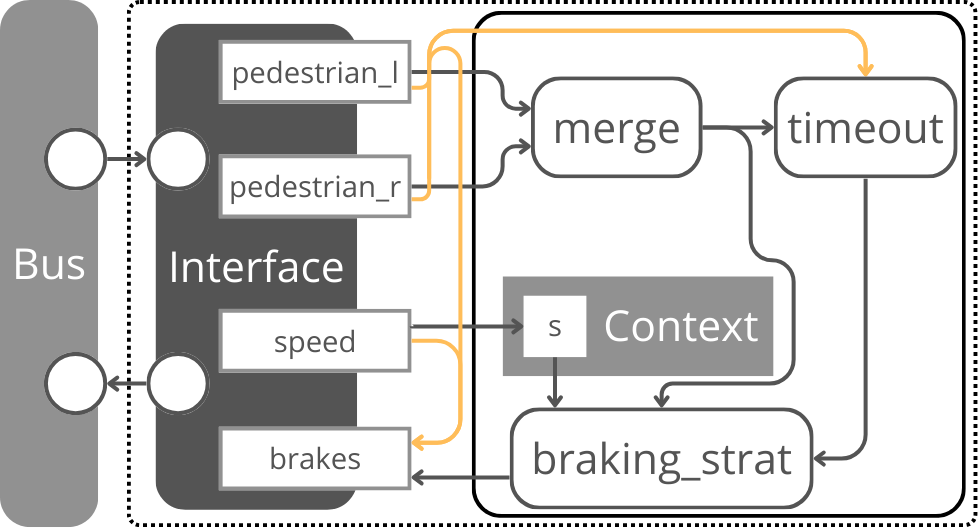
\includegraphics[width=\textwidth]{../images/execution_aeb.png}
    \caption[Execution scheme of Automatic Emergency Braking.]%
    {Execution scheme of \aeb service.}
    \label{fig:semantics:example:aeb:execution}
  \end{subfigure}
  \qquad
  \begin{subfigure}[b]{0.57\textwidth}
    \footnotesize
    \begin{tabular}{l|cccccc}
      \ttf{time}          & $t$           & $t + 1s$        & $t + 1.2s$    & $t + 1.5s$    & $t + 3s$      \\ \hline
      \ttf{speed}         & \changed{32.} & 32.             & \changed{30.} & \changed{25.} & 25.           \\
      \ttf{pedestrian\_l} &               & \changed{20.}   &               &               &               \\
      \ttf{pedestrian\_r} &               &                 &               &               &               \\
      \ttf{pedestrian}    &               & \updated{20.}   &               &               &               \\
      \ttf{t\_pedestrian} &               &                 &               &               & \updated{()}  \\
      \ttf{strat}         & \updated{\No} & \updated{\Soft} & \Soft         & \Soft         & \updated{\No}
    \end{tabular}

    Imports changes are red, local and export updates are blue.%
    \caption[Chronogram for the Automatic Emergency Braking.]%
    {Chronogram for the \aeb service.}
    \label{fig:semantics:example:aeb:chronogram}
  \end{subfigure}
  \caption[Automatic Emergency Braking example.]%
  {Automatic Emergency Braking (\aeb) example.}
  \label{fig:semantics:example:aeb}
\end{figure}

The execution of the \aeb service follows the scheme in \Cref{fig:semantics:example:aeb:execution}:
it propagates signal changes and event occurrences through the statements to maintain up-to-date and
consistent flows. Incoming flows are timestamped on-change/occurrence, allowing the \GRust operator
\kwf{timeout}, for instance, to emit the \idf{t\_pedestrian} event at the appropriate time by
counting time since the last occurrence of either of the pedestrian inputs. Though \kwf{timeout}
relies on an internal timer mechanism (expressed by the orange arrows), it produces normal events.

The chronogram in \Cref{fig:semantics:example:aeb:chronogram} illustrates the execution of the \aeb
service over time. Changes to imported values are shown in red, while updates to local and exported
values appear in blue. Execution begins at time $t$, when the vehicle's speed is updated. Since no
pedestrians are detected, no braking is initiated. At $t + 1s$, the left sensor detects a
pedestrian. This updates the merged \idf{pedestrian} event and resets the \kwf{timeout} timer to
$t + 1s + 2s$. The pedestrian event activates \idf{braking\_strat}, which evaluates the braking
distance and selects soft braking. This mode is then exported on the communication bus and
maintained until $t + 3s$. As no further pedestrian events occur within the 2-second timeout window,
the \kwf{timeout} event triggers at $t + 3s$, prompting \idf{braking\_strat} to switch back to no
braking. This change is exported again on the communication bus.

We stress that computations are triggered only when a flow changes/occurs and propagated through
equations only as far as flows change. The braking strategy is computed only when needed: when a
pedestrian is detected, when the timeout ticks, or when the vehicle's speed changes. This
on-change/occurrence strategy also applies to exported events and signals: if \idf{strat} had not
changed at $t + 3s$, nothing would have been sent through the bus.

\paragraph{\GRSync: component-modeling kernel}
%
Components in \GRust are defined using the \GRSync kernel, which models synchronous dataflow
behavior through reactive state machines operating over discrete time steps. Each component computes
its output flows based on its input flows at each instant, treating values as per-tick snapshots.
%
In the \idf{braking\_strat} component (\Crefrange{ex:line:brakingStart}{ex:line:brakingEnd}), the
inputs \idf{p} and \idf{t\_p} are of type \kwf{float?} and \kwf{unit?}, respectively. The \kwf{?}
suffix denotes an event input, which behaves like an optional value that is only present when the
event occurs. Signals (\eg \idf{s}) are always defined at every instant, while events may be absent.

Component behavior is specified using a set of unordered equations. \emph{Instantiations} assign
values to local identifiers or output flows (\Cref{ex:line:braking_distance}, \Cref{ex:line:braking}).
\emph{When equations} (\Crefrange{ex:line:whenStart}{ex:line:whenEnd}) define control points where
signal updates (\resp event emission) are triggered by event patterns. Those equations are analogous
to transitions in a state machine. For example, the component \idf{braking\_strat} initializes
\idf{b} to \No on \kwf{init} (\Cref{ex:line:when_init}), updates it to a new braking strategy
when a pedestrian is detected (\Cref{ex:line:brakes_call}), and resets it to \Soft or \No on timeout
(\Cref{ex:line:last,ex:line:t_p}). Event patterns like \detect{x}{p} (\Cref{ex:line:brakes_call})
bind the occurrence value of \idf{p} to an identifier \idf{x} that is local to the branch. If no
event occurs, the defined signals (or events) remain unchanged (or absent).

The \emph{operational} semantics of a component like \idf{braking\_strat} is defined as a
state machine. Its state holds the last value of some signals---here, the braking strategy
\idf{b}---initialized at time zero to \No. On each logical instant, the component reacts to
the current input values and produces outputs accordingly. For instance, the step function
\opsem{S, I}{\idf{braking\_strat}}{S', O}, from the state $S=\No$ and with the input values
$I=\{\idf{s}=32., \idf{p}=\some{20.}, \idf{t\_p}=\none\}$ produces a new state
$S'=\Soft$ and output values $O= \{\idf{b}=\Soft\}$.
The execution is guaranteed to be reactive and memory-safe: all computations terminate in bounded
time and use bounded memory, statically verified at compile time.

In the \emph{denotational} semantics, components are modeled as functions over streams.
A clock, represented as a stream of booleans, governs the timing of these streams. We say
a clock \emph{ticks} when its value is \true. Each stream defined on a clock has a value
at every tick.
%
Events, such as \idf{p} and \idf{t\_p}, are represented as streams of optional values,
where an occurrence is wrapped in \ttf{some} and an absence is marked by \none. The output
stream, \eg \idf{b}, is computed by applying the component equations at each clock tick.
The behavior of the \idf{braking\_strat} component is formally expressed as:
\begin{equation*}
  ck \vdashSync \idf{braking\_strat}[\idf{p}, \idf{t\_p}, \idf{s}] \Downarrow [\idf{b}],
\end{equation*}
This judgment states that on a given clock $ck$, the component transforms the input
streams \idf{p}, \idf{t\_p}, and \idf{s} into the output stream \idf{b}.
%
To illustrate, let us consider the execution trace from
\Cref{fig:semantics:example:aeb:chronogram}, assuming the clock $ck$ is always \true.
The first values of the streams for the application in \Cref{ex:line:strat} are:%
\setlength{\arraycolsep}{2pt}%
\begin{equation*}
  \begin{array}{rrlllllllllll}
    \idf{p}    & = & \none & \step & \some{20.} & \step & \none & \step & \none & \step & \none     & \cdots \\
    \idf{t\_p} & = & \none & \step & \none      & \step & \none & \step & \none & \step & \some{()} & \cdots \\
    \idf{s}    & = & 32.   & \step & 32.        & \step & 30.   & \step & 25.   & \step & 25.       & \cdots \\
    \idf{b}    & = & \No   & \step & \Soft      & \step & \Soft & \step & \Soft & \step & \No       & \cdots
  \end{array}
\end{equation*}%
\setlength{\arraycolsep}{5pt}%
%
The denotational view abstracts away the control flow of evaluation and focuses on the functional
relationship between input and output streams.

\paragraph{\GRFRP: service-modeling kernel}
%
Services are specified in \GRFRP, defining computations over data \emph{flows}.
These flows are classified as \emph{signals}, representing continuously evolving values like
vehicle speed, or \emph{events}, capturing discrete occurrences like pedestrian detection.

The code in \Cref{fig:semantics:example:aeb:code} defines the service \idf{aeb}
(\Crefrange{ex:line:aebStart}{ex:line:aebEnd}).
It imports the signal \idf{speed} and the events \idf{pedestrian\_l} and \idf{pedestrian\_r}
(\Crefrange{ex:line:importSpeed}{ex:line:importPedestrians}) from the communication bus.
It then defines local flows:
the event \idf{pedestrian} % is the union of the left and right detections
(\Cref{ex:line:pedestrian});
the event \idf{t\_pedestrian} % occurs when \idf{pedestrian} has not occurred for two seconds
(\Cref{ex:line:timeout});
and the signal \idf{strat} is the braking strategy computed by the component \idf{braking\_strat}
from the inputs \idf{pedestrian}, \idf{t\_pedestrian}, and \idf{speed} (\Cref{ex:line:strat}).
The signal \idf{strat} is then exported on the communication bus (\Cref{ex:line:export}).
%
Flows in \GRFRP are defined using both built-in operators from the \GReact library and
user-defined components written in \GRSync. For instance, the built-in operator
\kwf{merge} (\Cref{ex:line:pedestrian}) combines the two pedestrian detection events into a single
event, while \kwf{timeout} (\Cref{ex:line:timeout}) emits an event if \idf{pedestrian} has not
occurred for two seconds.

The \emph{operational} semantics of services models how they process incoming timestamped messages,
whether from external sources (\eg sensors, or other services) or internal mechanisms (timers).
Messages from external sources represent signal updates or event occurrences. The service reacts to
one incoming message at a time: it updates its internal state and timer queue, and produces any
relevant output updates.
%
In the \aeb example from \Cref{fig:semantics:example:aeb}, the internal state tracks the last value of the
output signal \idf{strat}, while the timer queue maintains the scheduled timeouts, \ie the timer
\idf{t_p} associated with \idf{t\_pedestrian}.
%
We illustrate the operational behavior of the \idf{aeb} service using a sequence of transition
steps. The state is represented as a pair $(S, \tau)$, where $S$ is the last value of \idf{strat} and
$\tau$ is the queue of timers containing \idf{t_p}. The transition relation
$(S, \tau) \xRightarrow[]{m,\,t} (S', \tau'): [(\idf{strat},v)]$ denotes that message $m$ is received
at time $t$, yielding the new state $(S', \tau')$ and possibly producing an update of the signal
\idf{strat} with value $v$. The following sequence corresponds to the execution illustrated in
\Cref{fig:semantics:example:aeb:chronogram}:
\begin{align*}
  (\No, \queue{(\idf{t_p},t_0)}) & \xRightarrow[\service{\kwf{aeb}}{\dots}]{\inputMess{\idf{speed}}{32.}, \, t} (\No, \queue{(\idf{t_p},t_0)}): [(\idf{strat}, \No)]                \\
                                 & \pushright{\text{\footnotesize Speed is updated, braking remains inactive.}}                                                                     \\
                                 & \xRightarrow[\service{\kwf{aeb}}{\dots}]{\inputMess{\idf{pedestrian\_l}}{20.}, \,t+1s} (\Soft, \queue{(\idf{t_p},t+3s)}): [(\idf{strat}, \Soft)] \\
                                 & \pushright{\text{\footnotesize A pedestrian is detected on the left. Timer reset to $t+3s$. Soft braking starts.}}                               \\
                                 & \xRightarrow[\service{\kwf{aeb}}{\dots}]{\inputMess{\idf{speed}}{30.}, \, t+1.2s} (\Soft, \queue{(\idf{t_p},t+3s)}): \emptylist                  \\
                                 & \pushright{\text{\footnotesize Speed changes, but braking remains soft. No update emitted.}}                                                     \\
                                 & \xRightarrow[\service{\kwf{aeb}}{\dots}]{\inputMess{\idf{speed}}{25.}, \, t+1.5s} (\Soft, \queue{(\idf{t_p},t+3s)}): \emptylist                  \\
                                 & \pushright{\text{\footnotesize Speed changes again. Braking logic is recomputed but result is unchanged.}}                                       \\
                                 & \xRightarrow[\service{\kwf{aeb}}{\dots}]{\timerMess{\idf{t_p}}, \, t+3s} (\No, \queue{(\idf{t_p},t+5s)}): [(\idf{strat}, \No)]                   \\
                                 & \pushright{\text{\footnotesize No pedestrian seen for 2s. Timeout fires, braking stops.}}
\end{align*}
This trace highlights that computations are triggered only by changes or occurrences in input flows,
and propagated only when the result changes. For instance, although the speed changes at $t + 1.2$
and $t + 1.5$ seconds, the braking strategy remains \Soft, so no update is emitted. Similarly,
the timeout event at $t + 3s$ causes \idf{strat} to switch back to \No, which is then exported.
This propagation model ensures that the system avoids unnecessary computations and communications
when the output remains unchanged.

The \emph{denotational} semantics of \GRFRP models flows as timestamped streams: signals are streams
of timestamped value updates, while events are streams of timestamped occurrences. Each service
corresponds to a function from input timestamped streams to output timestamped streams, defined over
a common timestamped clock \tck. The clock \tck is a global sequence of timestamps,
recording all moments when some input or output flow changes or occurs. Each stream---whether signal
or event---is defined only at a subset of these timestamps. The clock itself is the union of all
timestamps appearing in the input and output streams.
%
Given a timestamped clock \tck and streams \idf{speed}, \idf{pedestrian\_l}, \idf{pedestrian\_r},
and \idf{strat}, the judgment:
\begin{equation*}
  \tck \vdashFrp \idf{aeb} [\idf{speed}, \idf{pedestrian\_l}, \idf{pedestrian\_r}] \Downarrow [\idf{strat}],
\end{equation*}
denotes that the \idf{aeb} service evaluates over the timestamps in \tck and produces the
output stream \idf{strat} from the input streams \idf{speed}, \idf{pedestrian\_l}, and \idf{pedestrian\_r}.
For instance, the following timestamped clock and streams correspond to the execution illustrated in
the chronogram of \Cref{fig:semantics:example:aeb:chronogram}:
\begin{align*}
  \tck                & = (t, \true) \step (t+1s, \true) \step (t+1.2s, \true) \step (t+1.5s, \true) \step (t+3s, \true) \cdots \\
  \idf{speed}         & = (t, 32.) \step (t+1.2s, 30.) \step (t+1.5s, 25.) \cdots                                               \\
  \idf{pedestrian\_l} & = (t+1s, 20.) \cdots                                                                                    \\
  \idf{pedestrian\_r} & = \cdots                                                                                                \\
  \idf{strat}         & = (t, \No) \step (t+1s, \Soft) \step (t+3s, \No) \cdots
\end{align*}
The output stream \idf{strat} reflects the input history in a purely functional manner, abstracting away
internal evaluation steps or timer mechanisms. The denotational semantics captures only the relation
between the inputs and outputs flows over the global timeline defined by \tck.

This section introduced the core semantic concepts of \GRust through a practical example.
We have seen how the operational semantics models the step-based computation of \GRSync
components and the event-driven execution of \GRFRP services. The denotational semantics,
in turn, provides a higher-level view by modeling dataflows as streams. In \GRSync, these
are streams of values synchronized on a logical clock; in \GRFRP, they are streams of
timestamped values on a global timeline. To formally define these behaviors, we must first
establish a precise mathematical framework. The next section introduces the theory of
streams and clocks that provides this foundation.
